\chapter{Vector Spaces}
\begin{definition}
A vector space $V$ is a set of objects, such that any two objects can be added together, any object can be multiplied by a scalar. \\

If two objects belong to the vector space, then their sum also belongs to the vector space. \\

If an object belongs to $V$, then the product of any scalar with this object belongs to V and the following properties are satisfied:
\begin{enumerate}
\item $\forall \uv,\vv,\wv\in V$; $(\uv+\vv)+\wv = \uv+(\vv+\wv)$
\item $\forall \uv,\vv\in V$; $\uv+\vv = \vv+\uv$
\item There exists unique elements $\ul{0}\in V$, such that $\forall\uv\in V$; $\uv + \ul{0} = \ul{0} + \uv = \uv$
\item For any $\uv\in V, \exists!(-\uv)\in V$, such that $\uv+(-\uv) = \ul{0}$
\item $\forall \uv,\vv\in V$; $\forall \alpha\in\R$; $\alpha(\uv+\vv) = \alpha\uv + \alpha\vv$
\item $\forall \uv\in V$; $\forall \alpha,\beta\in\R$; $(\alpha+\beta)\uv = \alpha\uv + \beta\uv$
\item $\forall \uv\in V$; $\forall \alpha,\beta\in\R$; $(\alpha\beta)\uv = \alpha(\beta\uv)$
\item $\forall \uv\in V$; $1\cdot \uv = \uv$ (1 is a scalar here)
\end{enumerate}
\end{definition}
\begin{remark}
The ``vectors'' in the vector space, are not necessarily vectors ($\in\R^n$)	, but can be other objects, as long as the definition is satisfied.
\end{remark}

\begin{example}
Let us consider a set of all $2\times 2$ matrices. It is a vector space. Proof:
\begin{align*}
&\text{If }A,B\in\R^{2,2}\Rightarrow (A+B)\in\R^{2,2}\\
&\text{If }\alpha\in\R, A\in\R^{2,2}\Rightarrow\alpha A \in \R^{2,2}
\end{align*}

\begin{enumerate}
\item $A,B,C\in\R^{2,2}$; $(A+B)+C = A+(B+C)$
\item \dots 
\item \[
\ul{0} = \begin{pmatrix}
0 & 0\\
0 & 0
\end{pmatrix}\in \R^{2,2}, \forall A = \begin{pmatrix}
a_{11} & a_{12}\\
a_{21} & a_{22}\\
\end{pmatrix} \Rightarrow A+\ul{0} = A
\]
\item \[
A = \begin{pmatrix}
a_{11} & a_{12}\\
a_{21} & a_{22}\\
\end{pmatrix}\Rightarrow (-A) = \begin{pmatrix}
-a_{11} & -a_{12}\\
-a_{21} & -a_{22}\\
\end{pmatrix}
\]
\end{enumerate}
\end{example}
\todo[inline]{The layout of this example is not clear}
\begin{example}
Let us consider a set consisting of a single object, \ul{0}. It is a vector space. 
\end{example}

\begin{note}
There is no vector space, which does not contain $\ul{0}$	
\end{note}


\section{Subspace of the vector space}
\begin{definition}
A subspace $W$ of the vector space $V$, is a set of vectors in $V$, such that:
\begin{enumerate}
	\item If $\uv,\vv\in W$ then $\uv+\vv\in W$
\item If $\alpha \in\R$, $\uv\in W$ then $\alpha \uv\in W$
\end{enumerate}
\end{definition}
\begin{definition}
Let us consider a set of vectors $\{ \uv_1,\dots,\uv_n \}$. The span of vectors $\{ \uv_1,\dots,\uv_n \}$ is defined as
\[ \mathcal{S} = \text{span}\{\uv_1,\dots,\uv_n\} = \{\alpha_1\uv_1+\dots+\alpha_n\uv_n\mid \forall\alpha_1\dots\alpha_n\in\R\}\]
\end{definition}

\begin{example}
Is $\text{span}\{\uv\}$ a subspace in $\R^2$? Proof: 
\begin{align*}
\vv &= \alpha\uv\in\text{span}\{\uv\}\\
\wv &= \beta\uv\in\text{span}\{\uv\}\\
\end{align*}
\begin{enumerate}
\item $\vv+\wv=\alpha\uv+\beta\uv=(\alpha+\beta)\uv\in\text{span}\{\uv\}$
\item $\gamma\in\R,\gamma\vv=\gamma\cdot(\alpha\uv)=(\gamma\cdot\alpha)\uv\in\text{span}\{\uv\}$
\end{enumerate}

	
\end{example}


\begin{example}
\begin{enumerate}
\item \leavevmode\vadjust{\vspace{-\baselineskip}}\newline\begin{center}
\begin{tikzpicture}[scale=0.5]
\draw[<->] (-4,0) -- coordinate (x axis mid) (4,0) node[anchor=west]{$x_1$};
\draw[<->] (0,-4) -- coordinate (y axis mid) (0,4) node[anchor=south]{$x_2$};
\draw(-3.5,-3.5) -- (3.5,3.5);
\draw[very thick,->](0,0) -- (1,1)node[anchor=west]{$\uv$};
\draw[<-](2.2,2) --(2.7,2) node[anchor=west]{$\text{span}\{\uv\}$};
\draw (2,4) node {$\R^2$};
\end{tikzpicture}
\end{center}
\item \leavevmode\vadjust{\vspace{-\baselineskip}}\newline\begin{center}
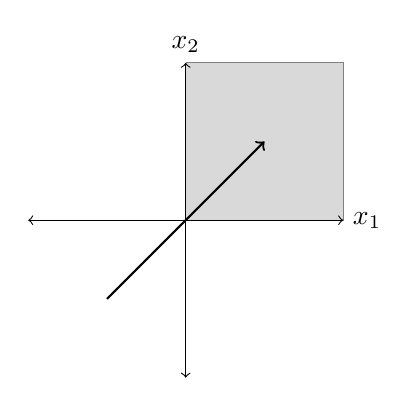
\begin{tikzpicture}[scale=0.5]
\draw[color=gray,fill=black!15] (0,0)--(4,0)--(4,4)--(0,4);
\draw[<->] (-4,0) -- coordinate (x axis mid) (4,0) node[anchor=west]{$x_1$};
\draw[<->] (0,-4) -- coordinate (y axis mid) (0,4) node[anchor=south]{$x_2$};
\draw[thick,->](-2,-2) -- (2,2);
\end{tikzpicture}
\end{center}
\item \leavevmode\vadjust{\vspace{-\baselineskip}}\newline\begin{center}
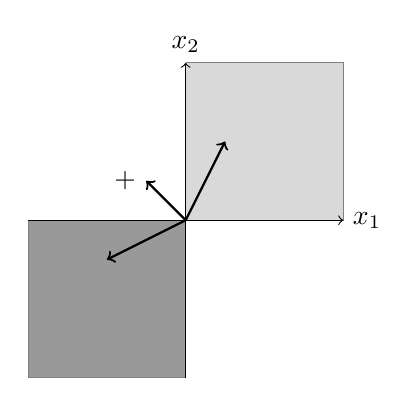
\begin{tikzpicture}[scale=0.5]
\draw[color=gray,fill=black!15] (0,0)--(4,0)--(4,4)--(0,4);
\draw[color=gray,fill=black!40] (0,0)--(-4,0)--(-4,-4)--(0,-4);
\draw[->] (-4,0) -- coordinate (x axis mid) (4,0) node[anchor=west]{$x_1$};
\draw[->] (0,-4) -- coordinate (y axis mid) (0,4) node[anchor=south]{$x_2$};
\draw[thick,->](0,0) -- (1,2)node[anchor=west]{$\uv$};
\draw[thick,->](0,0) -- (-2,-1)node[anchor=east]{$\vv$};
\draw[thick,->](0,0) -- (-1,1)node[anchor=east]{$\uv+\vv$};
\end{tikzpicture}
\end{center}
\end{enumerate}
\end{example}

\section{Linear Independence}
\begin{definition}
Let us consider vector space $V$ and $\vv_1,\dots,\vv_n\in V$. $\vv_1,\dots,\vv_n$ are linearly dependent if there exists scalars $\alpha_1,\dots,\alpha_n$ not all equal to zero, such that $\alpha_1\vv_1+\dots+\alpha_n\vv_n=\ul{0}$\\

If no such scalars exist, the vectors $\vv_1,\dots,\vv_n$ are linearly independent.
\end{definition}
\begin{definition}
Vectors $\vv_1,\dots,\vv_n\in V$ are linearly independent if the following is true:
\[
\alpha_1\vv_1+\dots+\alpha_n\vv_n = 0\Rightarrow \text{ all }\alpha_i = 0,i=1,\dots,n
\]
\end{definition}
\begin{example}
\begin{enumerate}
\item Let us consider $\R^n$ and vectors 
\[
\ul{E}_1 = \colvec{4}{1}{0}{\vdots}{0},\ul{E}_2 = \colvec{4}{0}{1}{\vdots}{0},\dots,\ul{E}_i = \colvec{4}{0}{1}{\vdots}{0},\ul{E}_n = \colvec{4}{0}{1}{\vdots}{0}
\]	
$\ul{E}_1,\dots,\ul{E}_n$ are linearly independent.
\item Let us consider $\R^2$, $\uv_1 = \colvec{2}{1}{1}$ and $\uv_2=\colvec{2}{3}{1}$. Are they linearly independent? See proof 2.
\end{enumerate}
\end{example}



\begin{proof}
\begin{enumerate}
\item Assume that
\[
\alpha_1\ul{E}_1+\dots+\alpha_n\ul{E}_n=0\Rightarrow \alpha_1\colvec{5}{1}{0}{0}{\vdots}{0}+\dots+\alpha_n\colvec{5}{0}{0}{\vdots}{0}{1} 
\]$\Rightarrow$ then all $\alpha_i=0$ for $i=1,\dots,n$,then based on the definition $\ul{E}_1,\dots,\ul{E}_n$ are linearly independent.
\item Let us consider $\alpha_1\uv_1+\alpha_2\uv_2 = \ul{0}\Rightarrow \alpha_1\colvec{2}{1}{1}+\alpha_2\colvec{2}{3}{1} = \colvec{2}{0}{0}$
\[
\begin{cases}
\alpha_1+3\alpha_2 = 0\\
\alpha_1+\alpha_2 = 0
\end{cases}\to\begin{cases}
2\alpha_2=0\\
\alpha_1+\alpha_2 = 0
\end{cases}\to\begin{cases}
\alpha_2=0\\
\alpha_1=0
\end{cases}
\]
If we assume $\alpha_1\uv_1+\alpha_2\uv_2 = \ul{0}$, we have to show that all $\alpha_i$ are zeroes $\Rightarrow$ vectors are linearly independent.
\end{enumerate}
\end{proof}

\begin{example}
Let us consider $\R^2$, $\uv_1=\colvec{2}{1}{1}$, $\uv_2=\colvec{2}{2}{2}$. Let us assume that 
\[
\alpha_1\uv_1+\alpha_2\uv_2=\ul{0}\Rightarrow \alpha_1\colvec{2}{1}{1}+\alpha_2\colvec{2}{2}{2} = \colvec{2}{0}{0}
\]
\[
\begin{cases}
\alpha_1+2\alpha_2=0\\
\alpha_1+2\alpha_2=0\\
\end{cases}\to\begin{cases}
\alpha_1+2\alpha_2=0\\
0=0\\
\end{cases}\]One possible solution:\[\begin{cases}
\alpha_1=-2\\
\alpha_2=1\\
\end{cases}
\]
Linearly dependent.
\end{example}
\begin{recap}
If we consider vectors $\vv_1,\dots,\vv_n\in V$, then
\[
\textbf{span}\{ \vv_1,\dots,\vv_n\} = \left\{\alpha_1\vv_1,\dots,\alpha_n\vv_n\mid\text{ for all possible }\alpha_1,\dots,\alpha_n\in\R \right\}
\]	
\end{recap}
\begin{definition}
If vector space $v$ is generated by $\{\vv_1,\dots,\vv_n\}$ (in other words, $V=\text{span}\{\vv_1,\dots,\vv_n\}$) and $\vv_1,\dots,\vv_n$ are linearly independent, then $\{\vv_1,\dots,\vv_n\}$ is called basis of $V$
\end{definition}

\begin{example}
Let us consider $\R^n$ and $\ul{E}_1,\dots,\ul{E}_n$. They form basis of $\R^n$. 	
\end{example}
\begin{proof}
\begin{enumerate}
\item ``$V$ is generated by $\vv_1,\dots,\vv_n$''. Let us consider any vector $\uv\in\R^n$
\begin{align*}
\uv &= \colvec{3}{\uv_1}{\vdots}{\uv_n}\text{, we have}\\
\uv &= \colvec{3}{\uv_1}{\vdots}{\uv_n} = \uv_1\ul{E}_1+\dots+\uv_n\ul{E}_n \Rightarrow \R^n=\text{span}\{\ul{E}_1,\dots,\ul{E}_n\}
\end{align*}
\item ``Linear independence'' already proven before. 
\end{enumerate}
\end{proof}

\begin{example}
Let us consider $\R^2$ and $\uv_1=\colvec{2}{1}{1}$, $\uv_2=\colvec{2}{3}{1}$, is it a basis?
\begin{enumerate}
\item Is $\R^2=\text{span}\left\{ \colvec{2}{1}{1},\colvec{2}{3}{1} \right\}$? Let us consider an arbitrary vector $\vv=\colvec{2}{\vv_1}{\vv_2}\in\R^2$. We should check that there exists scalars $\alpha_1,\alpha_2$ such that 
\[
\vv = \alpha_1\uv_1+\alpha_2\uv_2\to\vv = \alpha_1\colvec{2}{1}{1}+\alpha_2\colvec{2}{3}{1} = \colvec{2}{\vv_1}{\vv_2}
\]
\[
\begin{cases}
\alpha_1+3\alpha_2 = \vv_1\\
\alpha_1+\alpha_2 = \vv_2\\
\end{cases}\to \begin{cases}
2\alpha_2 = \vv_1-\vv_2\\
\alpha_1+\alpha_2 = \vv_2\\
\end{cases}\to\begin{cases}
\alpha_2 = \frac{\vv_1-\vv_2}{2}\\
\alpha_1 = \vv_2-\frac{\vv_1-\vv_2}{2} = \frac{3\vv_2-\vv_1}{2}\\
\end{cases}
\]
\item $\uv_1,\uv_2=$ linearly independent (We showed it before).
\end{enumerate}
\end{example}

\begin{definition}
Let us consider vector space $V$ and vectors $\vv_1,\dots,\vv_n$ that form a basis of $V$. If vector $\ul{x}\in V$ can be written as $\ul{x} = x_1\vv_1 + \dots + x_n\vv_n$ then ($x_1,\dots,x_n$) are called the coordinates of $\ul{x}$ with respect to basis $\{v_1,\dots,v_n\}$
\end{definition}

\begin{theorem}
Let us consider vector space $V$ and $v_1,\dots,v_n$ that are linearly independent. Let us assume that $\ul{x} = \alpha_1v_1+\dots+\alpha_nv_n$ and $\ul{x} = \beta_1\vv_1+\dots+\beta_n\vv_n$, then
\[
\alpha_i=\beta_i\hspace{4mm}\forall i = 1,\dots,n
\] 
\end{theorem}
\begin{proof}
We have 
\[x=\alpha_1\vv_1+\dots+\alpha_n\vv_n = \beta_1\vv_1+\dots+\beta_n\vv_n \to (\alpha_1-\beta_1)\vv_1+\dots+(\alpha_n-\beta_n)\vv_n = \ul{0}
\]
Since $v_1,\dots,v_n$ are linearly independent $\Rightarrow \alpha_i = \beta_i$, $\forall i = 1,\dots,n$
\end{proof}

\begin{remark}
The coordinates of any vector $\ul{x}$ with respect to given basis $\{\vv_1,\dots,\vv_n\}$ are unique.
\end{remark}

\begin{theorem}
Let us consider vector space $V$. The number of vectors in any basis of $V$ is always the same.
\end{theorem}
\begin{remark}
The number of vectors in the basis of vector space $V$ is called the dimension of vector space $V$.	
\end{remark}

\section{Rank of matrix}
\begin{definition}
The row rank of matrix A is a maximum number of linearly independent rows of matrix $A$.
\end{definition}
\begin{definition}
The column rank of matrix $A$ is a maximum number of linearly independent columns of matrix $A$.
\end{definition}

\begin{remark}
For any matrix $A\in\R^{m,n}	$, the row rank is equal to the column rank. Therefore the row rank and column rank are sometimes called rank of matrix $A$, $\rank(A).$
\end{remark}

\begin{example}
\begin{enumerate}
\item \[A = \begin{pmatrix}
1 & 3\\
1 & 1	
\end{pmatrix}
\]
We have shown before that $\colvec{2}{1}{1}$ and $\colvec{2}{3}{1}$ are linearly independent, therefore $\rank(A)=2$.
\item \[
A = \begin{pmatrix}
1 & 0\\
7 & 0\\
3 & 0\\
-1 & 0
\end{pmatrix} \in\R^{4,2}
\]
The column vectors $\colvec{4}{1}{7}{3}{-1}$ and  $\colvec{4}{0}{0}{0}{0}$ are linearly dependent, thus $\rank(A)=1$ (i.e. the maximum number of linearly independent columns is $1$).

\end{enumerate}
\end{example}

\begin{remark}
Two vectors are orthogonal if $\langle\uv,\vv\rangle = \uv^T\vv = 0$ (they basically must be perpendicular, i.e. the angle between  $\uv$ and $\vv$ is 90 degrees).
\end{remark}
\begin{definition}
Two subspaces $U$ and $W$ of vector space $V$ are orthogonal, if $\forall \uv\in U$ and $\forall \wv\in W$, we have $\langle \uv,\wv\rangle = 0$
\end{definition}

\begin{definition}
Orthogonal complement of subspace $M$ of vector space $V$ contains every vector orthogonal to $M$. This subspace is usually denoted by $M^\perp$
\end{definition}

\begin{remark}
$\dim M+\dim M^\perp = \dim V$	
\end{remark}
\begin{example}
Consider $\R^3$
\begin{center}
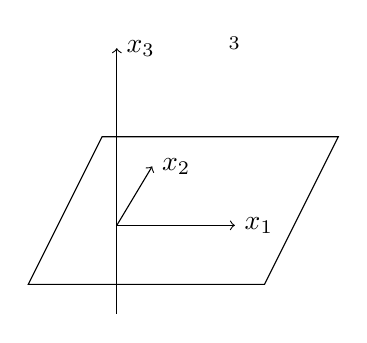
\begin{tikzpicture}[scale=0.75]
\draw[->] (0,0) -- coordinate (x axis mid) (2,0) node[anchor=west]{$x_1$};
\draw[->] (0,0) -- coordinate (x axis mid) (0.6,1) node[anchor=west]{$x_2$};
\draw[->] (0,-1.5) -- coordinate (x axis mid) (0,3) node[anchor=west]{$x_3$};
\draw[] (-1.5,-1) --(-0.25,1.5) --(3.75,1.5) -- (2.5,-1)--cycle;
\draw (2,3)node{$\R^3$};
\end{tikzpicture}
\end{center}
line $\alpha$ plane	- orthogonal subspace. Orthogonal complement of each other
\end{example}
\begin{example}
Not orthogonal subspace!\\
\adjustbox{valign=t}{
\begin{minipage}{0.3\linewidth}
$\uv\not=0$\\
$\uv\in I \hspace{2mm}\& \hspace{2mm}\uv\in W$\\
$\langle \uv\in U,\uv\in W\rangle=0$
\end{minipage}}
\hfill
\adjustbox{valign=t}{
\begin{minipage}{0.6\linewidth}

\begin{center}
\begin{tikzpicture}[scale=0.8]

\node [] (0) at (-2.5, 3) {};
\node [] (1) at (-2.5, 0) {};
\node [] (2) at (2.5, 0) {};
\node [] (3) at (2.5, 3) {};
\node [] (4) at (1.5, 4) {};
\node [] (5) at (-3, 1) {};
\node [] (6) at (-3, -2) {};
\node [] (7) at (1.5, 1) {};
\node [] (8) at (-2.5, 1.25) {};
\node [] (9) at (0, 0) {};
\node [] (10) at (1.5, 3) {};
\node [] (11) at (0, 3) {};
\draw [] (3.center) to (0.center);
\draw [] (2.center) to (3.center);
\draw [] (4.center) to (5.center);
\draw [] (5.center) to (6.center);
\draw [] (9.center) to (6.center);
\draw [] (0.center) to (8.center);
\draw [] (2.center) to (9.center);
\draw [dashed] (9.center) to (1.center);
\draw [dashed] (1.center) to (8.center);
\draw [] (4.center) to (10.center);
\draw [dashed] (10.center) to (7.center);
\draw [dashed] (7.center) to (9.center);
\draw [thick] (9.center) to (11.center);
\draw (0,1.5) node[anchor=west] {$\uv$};
\draw (2.5,2.75) node[anchor=east] {$u$};
\draw (1.5,3.5) node[anchor=east] {$w$};
\draw (0.25,0) -- (0.05,-0.15)-- (-0.22,-0.15); 
\end{tikzpicture}
\end{center}	
\end{minipage}}
\end{example}

\begin{note}
If vector $\uv$ belongs to 2 orthogonal subspaces, this vector is necessarily a zero vector, $\uv = 0$ because we should have 
\[
\langle\uv,\uv\rangle = \uv^T\uv = 0\Rightarrow \uv = \ul{0}
\]
\end{note}

























